\section{Simulation Results and Discussion}

\subsection{Constant food and egg laying}
	\label{chap:constantFoodConstantLaying}
	The first iterative simulation run is based only on the equations of \textit{David S. Khoury et al.}\cite{khoury13}. As expected the hive stabilizes at an equilibrium point while the stored food increases infinitely (see graph \ref{chap:sim_R0_1}).

\subsection{Constant food, dynamic egg laying}
	\label{chap:constantFoodDynamicLaying}
	The second iterative simulation run was to see if the new laying function (Figure \ref{fig:dynLayingRate})  was working as intended. As a result the bee population does not stabilize at one point, it now describes a more natural periodic form with a population maximum around August and a minimum around February.\\
	
	The colony we simulated did not survive with any daily mortality rates higher than 0.1. There are not enough bees emerging from the pupa stadium in order to compensate the mortality rate. However, we found that the new mortality rates assumed in our simulation (0.075 daily mortality) are still realistic. \textit{Henry et al.} \cite{henry12} describe mortality rates between 0.102 and 0.316 in empirical testing, which is the range in which \textit{Khoury et al.} \cite{khoury13} simulated. \textit{R. Dukas} \cite{dukas08} observed that mortality of foragers is in this range mainly because of predation. As we apply the mortality to all days, even in times and seasons without foraging (all bees stay in the hive), our simulated mortality rates are naturally lower.\\
	
	The stored food still increases infinitely, as the everyday income per forager bee is constant (see graph \ref{chap:sim_R0_2}).

\subsection{Environmental model}
	\label{chap:environmentalModelDiscussion}
	For testing the environmental model, we decided to change the quality indicator and delay seasons (especially autumn). The map (see chapter \ref{chap:mapFlowerPatchQuality}) is always a randomly generated map with equally distributed flower patches across the map and normal distributed flower patch quality. All other parameters are kept fixed so that the results are unambiguous.
	
\subsection{Empirical data based runs}
	In this run we wanted to see if our model can produce the same results as \textit{T.D. Seeley's} experiments from \textit{Wisdom of the hive} p. 44, Figure  2.14, year 1982. Our graphs in \ref{chap:sim_R1_1} correlate well with the empirical data (before a swarm leaves the hive). As swarming was never a part of our model, we're satisfied with the accuracy of the results. Furthermore, we could compare the graphs only visually, since \textit{T.D. Seeley} did not publish any  extensive numerical data of his empirical evidence.\\
	Compared to our earlier simulations, the food collection rate is now dominated by the availability of flowers and the forager count.
	
	\subsubsection{Typical simulated day (environment interaction)}
		The analysed day number 158 represents a peak in summer flower blooming, so we can easily extract some information. On a 'typical' summer day like this, the scout bees discover about $80\%$ of the patches after 2.5 hours. The rate at which the food is collected is increasing throughout the day, which is represented by the \textit{food collected change} graph in Figure \ref{fig:day158}. We attribute the fluctuating changes in the first 4 hours to the discovery of new patches and the first path optimizations taking effect. The change of collected food stabilizes as the path optimization has run it's course and no new food sources are discovered (see fig. \ref{fig:day158}).\\
		
		For the statistical analysis of this summer day, we've averaged the values and calculated the standard deviations for every parameter captured during an environment simulation (see fig. \ref{fig:day158variation}). The 20 runs needed for chapter \ref{chap:variationsOnAutumnFlowers} were used as data basis. For spring and autumn, the plots would look approximately the same because an equal distributed flower map is used. This means the same optimizations and scouting behaviours are expected.\\
		High correlation can be found between the amount of discovered patches and the slope/change of food income (linear correlation coefficient of 0.9263). This was expected, because with a higher count of discovered patches, bees are able to figure out the best ones and increase their income.\\
		A little less correlated, but still significant is the amount of active foragers to food income (linear correlation coefficient of 0.8767). The least significant correlation is found between active scouts and food income (linear correlation coefficient of 0.5076). This makes sense since scouts are not collecting food, only discovering flower patches.\\
		In figure \ref{fig:day158} and \ref{fig:day158variation}, the scout and forager count lower a bit in the middle of the day, between 10:30 and 16:30. The food income change directly reacts to this. This change in active bees exists because we selected the daily activity curve of the bees this way, according to \textit{T.D. Seeley's} empirical data (\textit{Wisdom of the Hive}, p. 86, fig. 5.2. \cite{seeley95}).\\
		
		The standard deviations are not significant for the discovered flower patches because with the high amount of scouts on this particular day (about 6\% of 20~000 bees), most of the introduced randomness is compensated (random walk, see chapter \ref{chap:randomWalk}).\\
		Active scouts and foragers vary a little, but mainly follow the activity curve we've chosen. The deviation is higher for scouts than for foragers because the amount of scouts is about 20 times smaller while the introduced variations happen in an absolute way (the balance between scouts and foragers can vary between two runs).\\
		Food income change has the highest deviation values because this is highly sensitive on how the bees select the waggle dances (see chapter \ref{chap:foragersDistribution}). However, over the day, the deviation becomes smaller because bees always optimize towards the highest food income. This is also reflected in the total food collected over the day: At the beginning, we observe low deviations. The highest values are found on the middle of the day. At the end of the simulated day, the deviation is close to non-existent.
		
		\begin{figure}[H]
			\centering
			\scalebox{.75}{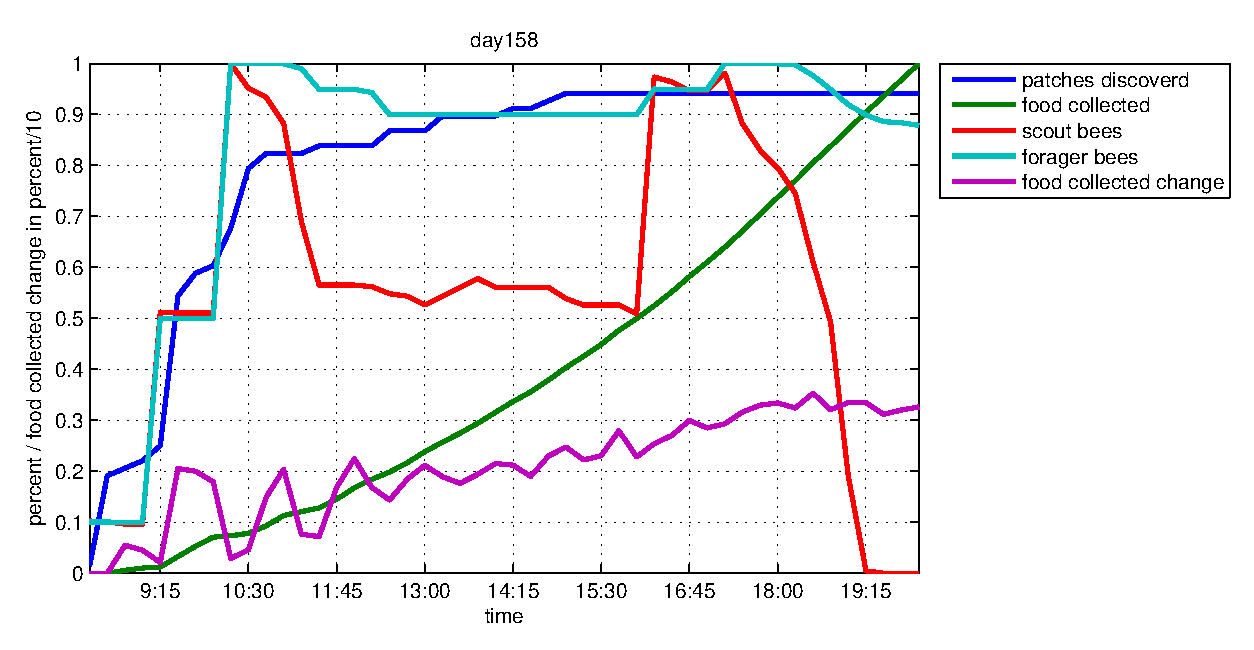
\includegraphics{../../code/results/Properties_Base_R1_1_day158.eps}}
			\caption{\textit{A summer day (day 158) from the standard run \ref{chap:sim_R1_1}. Values are given in fraction of the maximum value reached on day 158.}}
			\label{fig:day158}
		\end{figure}
		
		\begin{figure}[H]
			\centering
			\scalebox{.8}{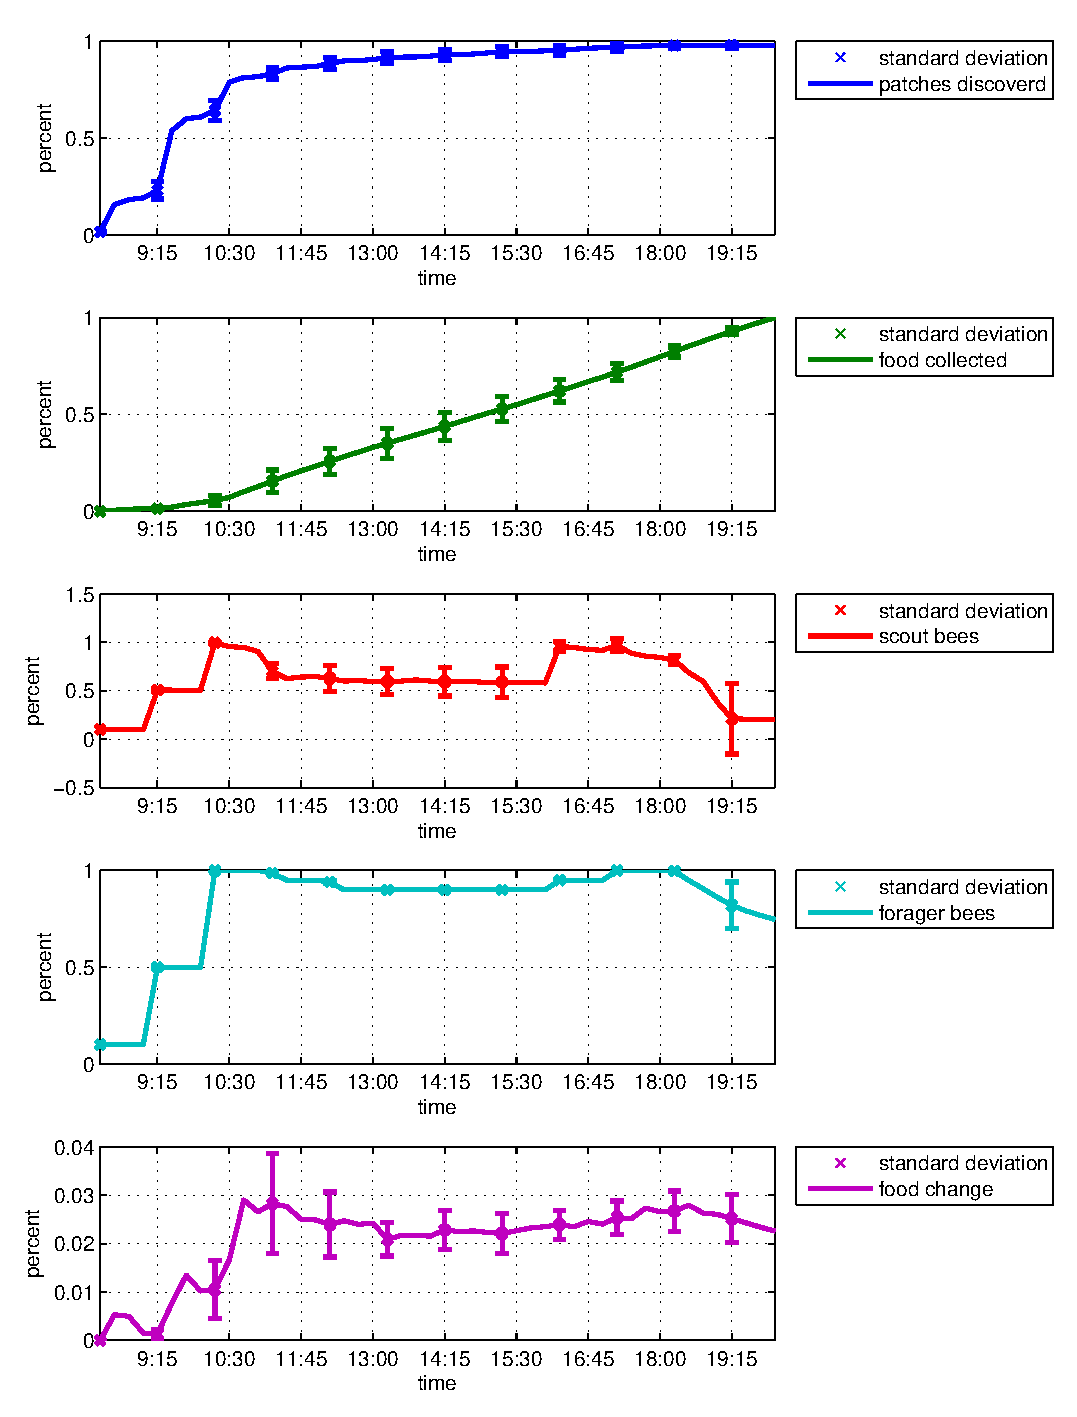
\includegraphics{../../code/results/Properties_Base_R2_variation_day158.eps}}
			\caption{\textit{A summer day (day 158), mean values over 20 runs from the standard run shown in appendix \ref{chap:sim_R1_1} with deviations. Values are given in fraction of the maximum value reached on day 158.}}
			\label{fig:day158variation}
		\end{figure}
	
	\subsubsection{Missing flower seasons}
		\label{chap:missingFlowerSeasons}
		In our first set of simulations (see \ref{chap:sim_R1}) we tested if any of the simulated blooming periods is not vital to the hive. We wanted to analyse the compensation mechanism of the hive and how the basic model interacts with the environmental simulation.\\
		
		We found out that when leaving out the spring blossom (see \ref{chap:sim_R1_2}), it doesn't necessarily lead to a critical situation in terms of food. The peaks of the stored food in summer were lower than those from the standard run \ref{chap:sim_R1_1}. We trace this back to the bee's ability to compensate the missing food income by consuming their stored food until summer.\\
		
		On the other hand, if summer or autumn are left out, the hive collapses. In the first case, the bees will survive the summer but the hive population dwindles to a level of about 1000 bees (see \ref{chap:sim_R1_3}). This is not sufficient to collect enough food in the autumn season and the hive dies. On day 200 (after all stored food is consumed) something very interesting happens: In order to survive, the bees stop taking care of the brood and eventually eat up the larvae (see equation \ref{eq:functionHiveBeesFood}, chapter \ref{chap:basicModel}). Because of the high need to get food, equation \ref{eq:changeForagers} of the basic model tries to recruit foragers from hive bees. From there on, both hive bee and forager numbers decrease as there is no brood to compensate mortality. On day 250, when the autumn season begins, not enough foragers are available and food, brood and bee numbers decrease monotonically.\\
		
		In case of a missing autumn food income (see \ref{chap:sim_R1_4}), the hive will starve as the bees consume the whole stored food before the winter really kicks in. Again, the bees try to compensate by assigning more foragers, which doesn't help and would be contra productive in a real world scenario (higher mortality of foragers and energy loss due to pointless foraging).
		By cannibalizing their brood, bees can help themselves trough short term lack of food (slightly delayed seasons or bad weather) but not through a whole missing seasons.
		
	\subsubsection{Variations on autumn flowers}
		\label{chap:variationsOnAutumnFlowers}
		The idea behind variations on autumn flowers was to see at which degree of delay or quality reduction the hive would start to collapse. For the quality indicator, we tested values between peak $M = 2.0\,\frac{kg}{day}$ and $M = 0.5\,\frac{kg}{day}$ (in steps of 0.5) for the autumn flowers (see fig. \ref{fig:seasonalFlowers} and chapter \ref{chap:flowerPatchesAndFood}). We delayed the season between 4 and 20 days (in steps of 4 days). More delay would shift the flowers into late autumn and winter, which makes no sense.\\
		We used 20~000 g and 1000 bees as the minimal requirement needed to survive in mid-winter. This values were picked in accordance with observations from the graph shown in appendix \ref{chap:sim_R1_1}: About 20~000 g of food is consumed from January to May to stabilize the hive and start brood reproduction to be ready for next summer's foraging. With less than 1000 bees, the hive can't fire up reproduction fast and reliable enough (see equation \ref{eq:functionHiveBeesFood} and chapter \ref{chap:basicModel}.)\\
		We found, that shifting the season by those 16 days has no significant effect on the forager count but probably on the flowers: They will lose blooming quality. Consequently, with $M = 0.5\,\frac{kg}{day}$ (see appendices \ref{chap:sim_R2_4_1} to \ref{chap:sim_R2_4_5}), the hive can not survive. The minimal stability point is around $M = 1\,\frac{kg}{day}$ (see appendices \ref{chap:sim_R2_3_1} to \ref{chap:sim_R2_3_5}). At this point, the variation of collected food over the year (see fig. \ref{fig:foodVariation}) becomes significant enough (3 to 5 kg) to affect the survival.\\
		%TODO: explain and elaborate more thoroughly. additionally, the last sentence is really hard to understand.
		
		Note that the standard deviation in Figure \ref{fig:foodVariation} basically sums up from the environment simulation (daily standard deviation of food income, see fig. \ref{fig:day158variation}). Therefore it only increases on foraging days, not during days without foraging, and does not decrease.
		
		\begin{figure}[H]
			\centering
			\scalebox{.75}{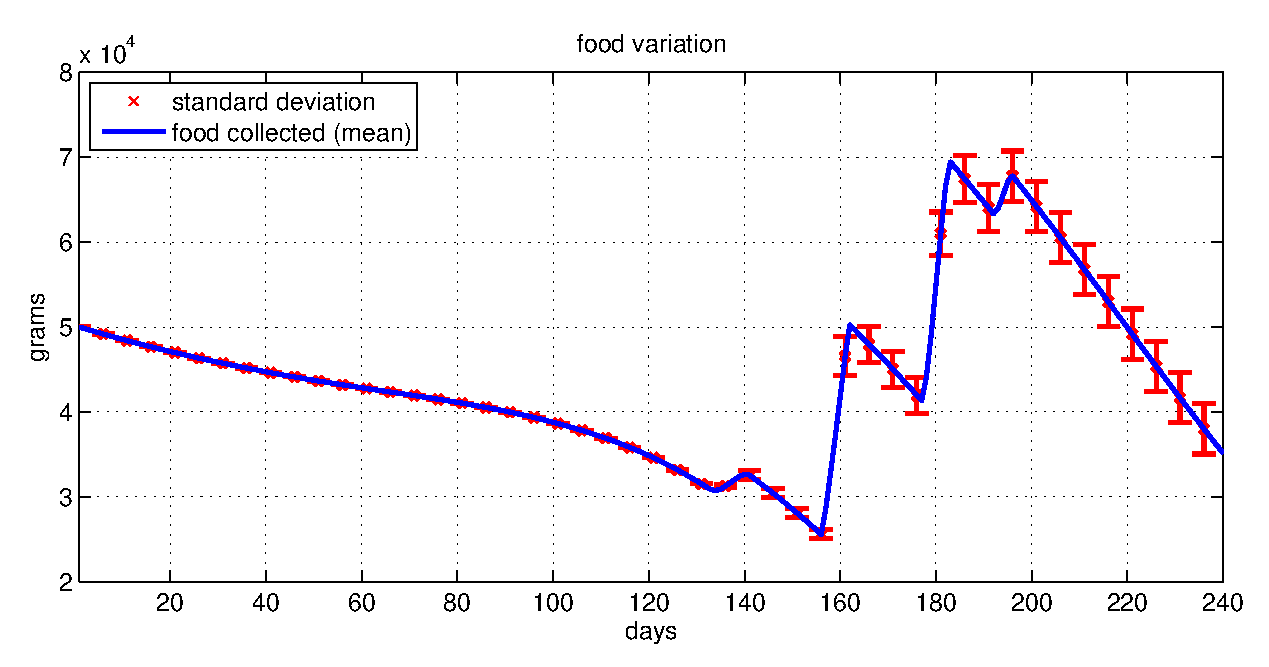
\includegraphics{../../code/results/Properties_Base_R2_food_variation.eps}}
			\caption{\textit{Food variation from January to August, mean values over 20 runs from the standard run shown in appendix \ref{chap:sim_R1_1} }}
			\label{fig:foodVariation}
		\end{figure}
	
	\subsubsection{Model restrictions}
		\label{chap:modelRestrictions}
		Even though we extended \textit{Khoury's} model by environmental influences on flowers and food reward, it is far from complete. One big divergence from nature is the treatment of pollen and nectar as one. Pollen, which is the protein source, and nectar, which is the carbohydrate source, are actually collected by two different forager classes intra-colonially \cite{schmickl07}.\\  Another big source of disturbance are diseases, infections, predation and swarming. Impairments in different aspects of a bee's life and behaviour, caused by pesticides or genetic mutation is entirely left out. There are also no other environmental influences such as aridity, wetland or weather and no human influences. \\
		In the end, one has to simulate the bee's way of "thinking", which is still a long way to go or might never be fully understood, even for advanced apiology and neuroscience.
		
	
